\subsection{GrammarSQL (no article? should i remove)}

Sequence-to-sequence models for neural text-to-SQL typically perform token-level decoding and do not consider generating SQL hierarchically.

\begin{itemize}
    \item \cite{xu_sqlnet_2017} proposes a grammar-based model for reducing the complexity of Text-to-SQL tasks involving hierarchical grammars.
    \item The authors introduce schema-dependent grammar with minimal over-generation.
    \item The grammar developed in \cite{xu_sqlnet_2017} covers 98\% of the instances in ATIS and SPIDER datasets.
\end{itemize}

\subsubsection{SQL Grammar}

The shallow parsing expression grammar (PEG) aims to capture as little SQL as possible to cover most instances in the dataset. This makes it a versatile tool for handling a wide variety of SQL queries. To further ensure consistency of table, column, and value references in SQL, the authors added non-terminals to the context-free grammar to use these references for cross-table joins.

At runtime, constraints are used to guarantee that only valid programs can be used to join different tables in a database together using a foreign key. This ensures that the data stored in the database is kept consistent and that the integrity of the database is maintained.

\subsubsection{Few details on the proposed model}

\begin{itemize}
    \item As an input, the proposed model takes an utterance of natural language, a database, and grammar about that utterance.
    \item String matching heuristics are applied after taking the input to link words in the input to identifiers or tokens in the database.
    \item Afterward, the bidirectional LSTM receives a concatenated string of the learned word and the link embeddings for each token.
    \item Using the attention mechanism, the decoder builds up the SQL query iteratively on the input sequence.
    \item Database identifiers in natural language questions and SQL queries are also anonymized.
\end{itemize}

\begin{figure}[H]
    \centering
    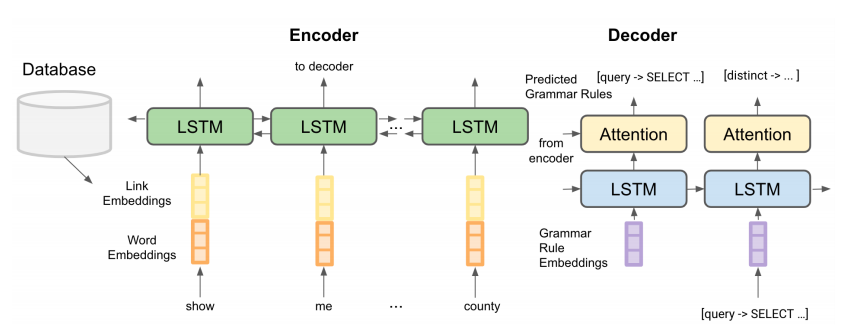
\includegraphics[width=0.8\textwidth]{pics/GrammarSQL.png}
    \caption{Structure of the proposed model}
    \label{fig:GrammarSQL}
\end{figure}


On ATIS and SPIDER datasets, the GrammarSQL model was evaluated. By 14\%, it outperformed SyntaxSQLNet, the previous SOTA model.